\chapter{Implementacja}
\label{cha:implementacja}

W niniejszym rozdziale zostanie bardziej szczegółowo opisana realizacja komponentów
gry opisanych w części \ref{cha:projekt}.

\section{Użyte narzędzia}
\label{sec:uzyteNarzedzia}

\subsection{Google Closure}
\label{ssec:googleClosure}

\section{Wielowątkowość}
\label{sec:wielowatkowosc}

\section{Główna pętla logiki gry}
\label{sec:logikaGry}

\section{Renderer}
\label{sec:renderer}

\section{Synchronizacja sieciowa}
\label{sec:synchronizacjaSieciowa}

\section{Zasoby gry}
\label{sec:zasobyGry}

\section{Opis z punktu widzenia użytkownika}

\begin{figure}[h]
  \centering
  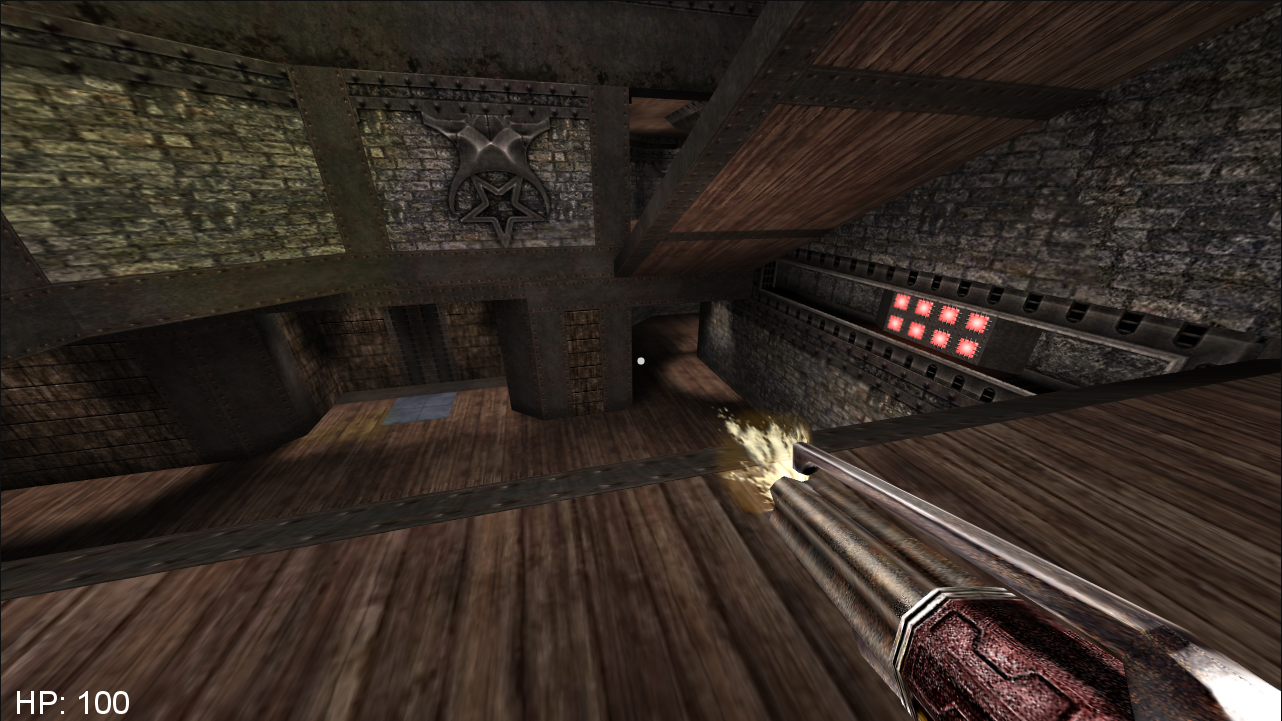
\includegraphics[scale=0.4]{zasoby/rozdzial31/screen}  
  \caption{Zrzut ekranu z gry Web Arena}
  \label{fig:screen}
\end{figure}


%%% Local Variables: 
%%% mode: latex
%%% TeX-master: "praca"
%%% End: 
